ALIAS was being developed using iterative approach. For each iteration a different approach for computing the extensions has been implemented. In order to verify and benchmark the approach, each iteration had allocated time for testing. Furthermore, the testing process can be divided into two separate processes: 
\begin{enumerate}
	\item Unit testing - number of tests created to verify the correctness of the proposed solution. Those tests are to verify if any change to the solution still produces correct output. 
	\item Benchmark testing - more extensive testing carried out at the end of each iteration. The purpose of the benchmark testing is to help evaluate the system. 
\end{enumerate}


As described in section \ref{label:projectRequirements}, there are number of functional and non-functional requirements for ALIAS. One of the most critical set of requirements identified are the correctness of computed solution and the scalability. In order to verify those requirements the black-box testing technique was used. Black box testing as described by \citet{testing2} is "based on the analysis of the specification of a piece of software without reference to its internal working". Hence, during the benchmark testing, the results were based on the output of the system and its response time. With no regards to the inner workings of the application, it allows examine only the fundamental workings of the system. Thus, in order to use the black-box testing, the final testing for each approach was done once the implementation was finished \citep{blackbox}.

In order to extensively test ALIAS, benchmark argumentation frameworks have been taken from the published sample argumentation frameworks from ICCMA 2017 \citep{iccmaResults}. The website provides 5 different sets of argumentation frameworks for all tasks involved in the competition and additional set for a Dung's Triathlon. Selected argumentation frameworks have been classified into 5 categories: very easy, easy, medium, hard and too hard. Appendix \ref{appendix:benchmarkFiles} shows the full list of argumentation frameworks used including the number of arguments and attacks. Although, different set of frameworks have been used for testing preferred and complete, and stable extensions, it can be seen that the sizes and complexity of the argumentation frameworks used differ. Starting from small framework including only 2 arguments and single attack the complexity increases to as much as six thousand arguments and over sixty thousand attacks in some cases. This is to help identify limits and possible issues with proposed solution. 

Additional benefit of using the benchmark frameworks from ICCMA 2017 competition is to be able to compare the results of ALIAS against the existing solutions. Furthermore, the benchmark testing can help identify the best solution and aid with improving the approach used. With satisfactory results, ALIAS could take a part in the future competitions.

\subsection{Unit testing}
Unit tests played important role during the development of each approach for ALIAS. Every change to the proposed solution has been tested and verified by using small number of argumentation frameworks. Each framework has been created and tested using other systems like Pyglaf and ArgSemSAT to ensure the outputted extensions are correct. 

Although unit testing does not help with evaluating the overall performance of ALIAS it played critical role during the development of the system. 

\subsection{Performance}
As \citet{performanceTesting1} points out the performance requirements play a key role in determining the usability and quality of many systems. In case of ALIAS the biggest concern in terms of performance is scalability. Argumentation frameworks used for unit testing were small in comparison to frameworks used in real world application or competitions like ICCMA. Thus, to correctly evaluate the performance and abilities of ALIAS, the benchmark argumentation frameworks have been used.

In order to test the scalability and performance, each implemented solution has been put through extensive testing. For each extension implemented within the proposed solutions, tests have been executed using the appropriate argumentation frameworks from appendix \ref{appendix:benchmarkFiles}. Each test run has been executed on the same machine with following specifications:

\begin{itemize}
	\item Processor: Intel Core I5-6200U @ 2.30 GHz
	\item GPU: Nvidia GeForce 940MX
	\item RAM: 8GB
	\item OS: Linux based
\end{itemize}

Using the same specifications for each test run allows for the test results to be easily comparable. Furthermore, since ICCMA 2017 competition has been ran on a different machines, Pyglaf \citep{pyglaf} and ArgMatSAT \citep{argmatSat} have been put through the same benchmark testing. Those results were used to compare and evaluate the performance of ALIAS to the most successful solvers submitted to ICCMA 2017.

During the testing, the CPU time has been limited per each argumentation framework to 20 minutes. This is to prevent the solver from computing the extensions indefinitely, especially on larger and more complex argumentation frameworks. The time required to read and parse files was not included in the specified time limit and it was used purely for computing all extensions. 

There were four separate proposed solution for computing abstract argumentation. Three of them were using the same method of computing the maximal conflict free set, but using different data structures to overcome certain issues and limitations as described in section \ref{section:maxConflictFreeSet}. The final approach is using SAT solver to enumerate possible solutions (see section \ref{section:satSolver}). Each approach was generating a number of possible solutions, which were then verified using matrix approach for preferred extension and set inclusion for stable extension as shown in sections \ref{section:preferredExtension} and \ref{section:stableExtension} respectively. 

\subsubsection{Stable Extension results}

\begin{figure}[h]
	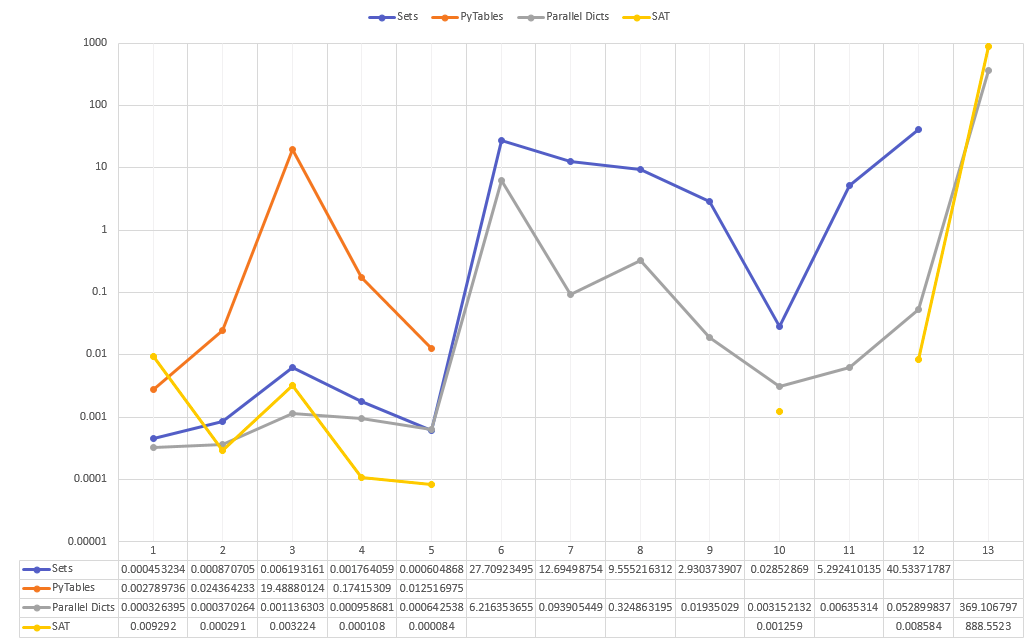
\includegraphics[width=\textwidth]{stable_results}
	\caption{Timings of 4 approaches computing Stable Extension}
	\label{fig:stableFinalResults}
\end{figure}

Figure \ref{fig:stableFinalResults} shows the execution times of all four approaches: sets, PyTables, parallel dictionaries and SAT solver for computing all Stable Extension on the set of argumentation frameworks specified in appendix \ref{appendix:benchmarkFiles}. The chart only shows the timings for the first 13 frameworks. Almost most of the approaches failed to produce the results for the remaining frameworks within the specified 20 minutes time limit. Furthermore, as can be seen in the chart \ref{fig:stableFinalResults}, certain data points are missing for some of the approaches. This is also due to the solver reaching a 20 minutes time limit without providing the solution. 

As can be seen in figure \ref{fig:stableFinalResults}, only approach using parallel dictionaries managed to compute the stable extensions for those frameworks in the specified time. Furthermore, it has the shortest execution time for majority of the frameworks across all approaches, with exception for five of them, where SAT solver approach considerably outperformed it. The execution time of dictionaries approach closely correspond to the approach using sets. Although sets operation are highly optimized in Python, it still did not outperform the implementation using dictionaries.

The worst performing solution is the PyTables approach to computing and storing the Maximal Conflict Free Sets. This approach only computed the extensions for first five argumentation frameworks provided, which had the lowest number of arguments and relations between them. Those results are due to dynamically creating the sets iterating through all the attacks within the argumentation framework as shown in section \ref{section:maxConflictFreeSet}. Since PyTables stores data on the hard drive, the read/write access creates high latency in terms of getting and storing values. This in turn has impact on the overall performance of the solution. 

Although the sets and dictionaries approaches for Maximal Conflict Free Sets creation produced results for most of the provided argumentation frameworks, they have a massive overhead - memory usage. The tests were performed on the machine with 8GB RAM available for the solver and another 8GB swap memory. Both of the solutions: sets and dictionaries, were running out of memory space for any framework with 20 or more arguments. Since this approach is combinatorial and generates all the possible maximal conflict free sets first, the number of combinations is extremely high. Hence, storing all possible sets is memory expensive as in the worst case scenario it will generate $2^n$ records, where $n$ is the number of arguments in the framework.

SAT based approach tends to outperform other solutions for frameworks it managed to complete the computation. As can be seen in figure \ref{fig:stableFinalResults}, half of the timings for SAT solver approach are considerably faster than other approaches. Only in 3 instances, this approach was slower than approach using dictionaries. However, as shown in the section \ref{section:satSolver}, SAT based approach uses a simple encodings for the admissible sets. Due to the size of argumentation frameworks used for testing, it caused the solver to reach the 20 minutes time out for 5 of the frameworks used for comparison. 

\subsubsection{Preferred Extension results}

\subsection{Correctness}
Correctness of the computed semantic is the critical functionality of the successful solver. However, this introduce the challenge of finding the best way to verify the produced solution. There are number of formal approaches that could be applied to the solver in order to confirm it provides the correct answer. For example, formal method called Z, "formal specification methodology that can dramatically improve the way software systems are modeled and implemented" \citep{potter1996introduction}, could be used to model the application and provide the proof of correctness. Although defining the approach and modeling the system could provide the guarantee for the correctness of the application, this is outside of the scope of this project. 

Thus, In order to test and verify the correctness of ALIAS, the same argumentation frameworks from appendix \ref{appendix:benchmarkFiles} have been used as for the performance testing. The outputs of the SAT based approach have been compared to the results of two winning solvers: Pyglaf \citep{pyglaf} and ArgSem-SAT \citep{argsemsat}. Although this does not guarantee the correct results, those solvers were the two highest scoring solvers in the competition and if their results are equal, the probability of answer being incorrect is low.
